\documentclass[a4,12pt,ngerman,listof=numbered]{scrartcl}
\usepackage[ngerman]{babel}
\usepackage[utf8]{inputenc}
\usepackage{listings}
\usepackage{float}
\usepackage{placeins}
\usepackage{minted}
\usemintedstyle{tango}
\usepackage[activate]{microtype}
\usepackage{amsmath}
\usepackage{graphicx}
\usepackage[colorinlistoftodos]{todonotes}
\usepackage{csquotes}
\usepackage{setspace}
\usepackage[margin=2.5cm]{geometry}
\usepackage[hidelinks]{hyperref}
\usepackage[backend=bibtex,style=numeric,sorting=none,date=long,hyperref=true]{biblatex} %sorting=none sorts by position of appearance
\usepackage{ulem}

\newcommand*{\qqquad}{\qquad\qquad\qquad\qquad}

\addbibresource{lit} 

\begin{document}

\begin{titlepage}

\newcommand{\HRule}{\rule{\linewidth}{0.5mm}}

\center

\textsc{\LARGE Karlsruher Institut für }\\[0.5cm]
\textsc{\LARGE Technologie} \\[1.5cm]
\textsc{\Large KASTEL Praktikum}\\[0.5cm]

\HRule \\[0.4cm]
{ \huge \bfseries Angriffe auf WPA2 PSK in der Praxis}\\[0.4cm] %TODO: Titel
\HRule \\[1.5cm]
 

\begin{minipage}{0.4\textwidth}
\begin{flushleft} \large
\emph{Autoren:}\\
Florian D. \textsc{Loch} \\
Benny \textsc{Görzig}
\end{flushleft}
\end{minipage}
~
\begin{minipage}{0.4\textwidth}
\begin{flushright} \large
\emph{Betreuer:} \\
Dr. Erik \textsc{Krempel}
\end{flushright}
\end{minipage}\\[2cm]


\includegraphics{logo}\\[1cm] 

{\large \today}\\[1cm]

\vfill 

\end{titlepage}

\newif\ifsigned
\signedtrue
% \signedfalse

\ifsigned
	\newpage
	\section*{Erklärung}
	Mit unseren Unterschriften bestätigen wir, dass die vorliegende Arbeit selbstständig verfasst und keine anderen als die angegebenen Quellen und Hilfsmittel verwendet wurden.\\
	
	% Zeile für Unterschrift
	\begin{flushleft}
		\uline{Ort:\qqquad\qqquad}\quad\uline{Datum:\qqquad\qqquad}\\
		\vspace{1cm}
		\uline{Florian Loch:\qqquad\qquad\qquad}\quad\uline{Benny Görzig:\qqquad\qquad\quad}
	\end{flushleft}
	\vfill
	\newpage
\fi

\normalem % corresponding to ulem changing emph

\tableofcontents

\newpage

\section{Motivation \& Einleitung}
Drahtlose Netzwerke, insbesondere IEEE 802.11, sind seit Jahren allgegenwärtig und werden in ihrer Bedeutung sicher noch weiter zunehmen. Egal ob in Büroräumen, in Universitäten oder dem eigenen Wohnzimmer - WLAN, ist nicht wegzudenken -- so verfügen viele Endgeräte mittlerweile auch gar nicht mehr direkt über tatsächliche Anschlüsse für kabelgebundene Netzwerke; ganze andere Klassen von Endgeräten wurden erst durch WiFis möglich bzw. nützlich: Smartphones, Tablets etc..

Wohl niemand hat ernsthafte Bedenken, wenn er in drahtlosen Netzen kommuniziert -- ungeschützte, öffentliche Hotspots einmal ausgelassen. Und dass, obwohl gerade diese Netze aus physikalischer Sicht besonders exponiert sind -- die schlichte Nähe zum Zugangspunkt genügt, um aktiv in die Kommunikation einzugreifen.

Doch durch entsprechenden Schutz auf Schicht zwei des ISO/OSI-Modells sollen Vertraulichkeit und Integrität aller darüberliegenden Protokolle transparent gewahrt werden.

Nachdem mit WEP ein nur unzureichendes Verfahren entwickelt und auf den Markt gebracht worden war, um diese Ziele umzusetzen, wurde mit WPA eine Teilmenge der damals in Entwicklung befindlichen \enquote{Robust Secure Network}-Spezifikation (RSN bzw. 802.11i TODO Quelle) als vorübergehender Standard verabschiedet. Seit 2004 ist der komplette RSN-Standard unter dem Namen WPA2 dabei, die alten Verfahren vollständig zu ersetzen.	

Bezüglich der grundlegenden, theoretischen Sicherheit von WPA2(-PSK) und den kryptographischen Primitiven gibt es in der Wissenschaft keinen Zweifel \footnote{2012 wurde das Verfahren nach 8 Jahren Einsatz weiterhin als sicher angesehen \cite{kumkar2012}, seitdem sind keine nennenswerten Schwachstellen gefunden worden.} -- diese Arbeit widmet sich daher der Frage, wie praxisrelevant Bruteforce-Angriffe auf WPA2-PSK sind, wie sie funktionieren und ob daher in der Praxis tatsächlich weiterhin sorglos auf 802.11i gesetzt werden sollte.

Hierfür werden nötige Grundlagen hinsichtlich IEEE 802.11 eingeführt, anschließend werden verschiedene Angriffsansätze zur Erlangung eines WPA2-PSK-Handshakes sowie das (versuchte) Brechen desselben beschrieben. Nach Besprechung der Praktikabilität wird in einem praktischen Kapitel die Durchführung dieser Angriffe in der Praxis mit konkreten Programmen aufgezeigt, um mit einer Zusammenfassung unserer Ergebnisse und einem Ausblick zu schließen.


\newpage

\section{Grundlagen}
Fokus eher auf WPA2/PSK
Wir werden natürlich nicht den vollständigen IEEE 802.11a, b, g, n und ac (...) Standard beschreiben, aber wichtige Grundlagen für die Angriffe
\subsection{Sicherheitsmechanismen bei 802.11}

\subsection{Management Frames}
Beacon Frames, Deauthentification Frames, Probe Requests/Responses

\subsection{WPA2}

\newpage

\section{Angriffe}
Im Rahmen dieser Ausarbeitung wollen wir uns auf die Ermittlung des \textit{Pre-shared Keys} (\textit{PSK}) als Angriffsziel und auf den Angriffsvektor des Brechens mitgeschnitttener Handshakes durch Exploration des Schlüsselraumes (Bruteforce) beschränken.

Tatsächlich gibt es nach dem bekannten Stand der Forschung keine Schwachstellen im Protokoll von WPA2-PSK, die es einem, nicht der Nutzergruppe angehörenden, Angreifer ermöglichen würden, die Kommunikation zu entschlüsseln. Es gibt bspw. eine Schwachstelle (\enquote{Hole 196}), die die Ermittlung des PTKs anderer Teilnehmer ermöglicht -- allerdings muss dem Angreifer hierfür der PSK bekannt sein, was die praktische Relevanz des Angriffes drastisch reduziert.

Aufgrund der Aufmerksamkeit, der sich dieses Thema unter Netzwerkexperten und Kryptologen in der Vergangenheit erfreute, ist nicht damit zu rechnen, dass in dem Verfahren noch grundlegende Schwachstellen gefunden werden. 

Da die Sicherheit eines solchen Verfahrens jedoch von mindestens drei Dingen abhängt -- der Sicherheit des Protokolls sowie der kryptografischen Primitiven, der fehlerfreien Implementierung und auch der Wahl eines guten Geheimnisses -- reicht dies allein nicht aus. 
So liegt die Wahl des Geheimnisses (in diesem Fall des Netzwerkschlüssels) meist in der Hand des nicht zwingend sachverständigen Endnutzers. 
So kann ein schlecht gewähltes Passwort oftmals durch einen durchdachten Wörterbuchangriff in realistischer Zeit gebrochen werden, ohne das Protokoll als solches angreifen zu müssen.

Die im Standard beschriebenen Anforderungen an einen PSK legen lediglich eine Länge von 8 Zeichen fest. \cite{zviran1999password} zufolge wählen Nutzer im Mittel lediglich 6 Zeichen lange Passwörter und greifen darauf in 8 von 10 Fällen ausschließlich auf Buchstaben zurück. Nur 13,7 \% der in dieser Studie analysierten Passwörter waren alphanumerisch. Auch wenn man davon ausgeht, dass Privatanwender für ihr WLAN womöglich ein vergleichsweise langes Passwort wählen, da sie es nicht täglich eingeben müssen -- so werden sie vermutlich weiterhin auf Wörter oder gängige Wort-Zahl-Kombinationen zurückgreifen, um es bspw. einfach an Gäste weitergeben zu können.
Auch finden sich immer wieder Berichte über schlechte Standardpasswörter \cite{stanched2015defaultpasswords}, mit denen die Geräte seitens des Herstellers oder ISPs ausgeliefert werden. Die Hoffnung, auf ein schwaches Passwort zu stoßen ist daher keinesfalls unbegründet -- und wie später dargelegt werden soll, hängt die gesamte Sicherheit je nach Angriff vom am schwächsten gesicherten Netzwerk ab, dass dem Gerät bekannt ist.\\

Eine weitere Spielweise sind Social-Engineering-Angriffe, die auf Unwissenheit, Unaufmerksamkeit und Leichtgläubigkeit der Nutzer setzen. 
Durch die nachfolgend beschriebene \enquote{Auskunftsfreudigkeit} der meisten Endgeräte hinsichtlich ihrer bekannten Netzwerken ergeben sich für Tools dieser Kategorie Möglichkeiten ihre Angriffe plausibel und für die meisten Nutzer authentisch wirkend durchzuführen.
So strahlt zum Beispiel das Tool \textit{wifiphisher} über einen geeigneten Netzwerk-Adapter ein offenes Netzwerk mit beliebiger SSID aus und präsentiert verbundenen Nutzern je nach System verschiedene, teils täuschend echt aussehende Dialoge zur Eingabe des Netzwerkschlüssels. 
Um einen Nutzer in das eigene Netzwerk zu bringen nutzt das Tool den später beschriebenen Deauth-Angriff. 

\textit{Fluxion} prüft die vom Benutzer getätigten Eingaben zusätzlich gegen einen mitgeschnittenen Handshake ab und kann sich so dem Benutzer gegenüber authentisch Verhalten und Falscheingaben erkennen. 
Dieser und weitere Angriffe, wie sie beispielsweise in~\cite{caneill2010attacks} beschrieben sind, sollen in dieser Ausarbeitung jedoch nicht weiter betrachtet werden, da ihr Ansatz ein grundlegend anderer ist.\\

\subsection{Erfassen eines WPA2-Handshakes}
Bei Bruteforce-Angriffen unterteilt sich die Ermittlung des Netzwerkschlüssels (PSK) in zwei elementare Schritte: 
\begin{enumerate}
	\item Die Erfassung eines WPA2-PSK-Handshakes während der Authentifizierungsphase zwischen Client und AP
	\item Die nachgelagerte Suche nach einem Schlüssel, der zu einem gleichen \textit{Message Integrity Code} führt
\end{enumerate}
Die vermutlich subtilste Methode zur Erlangung eines Handshakes, die dem Angreifer zur Verfügung steht, ist die passive Überwachung des Netzwerkverkehrs.
Dafür muss er lediglich abwarten, bis sich ein Client gegenüber einem AP im gewünschten Netzwerk authentifiziert. 
Abhängig von der Netzwerkinfrastruktur und des Nutzungsverhaltens des Clients kann dies jedoch viel Zeit in Anspruch nehmen.
Da dies für einen gezielten Angriff nicht zielführend erscheint werden nachfolgend zwei Angriffe beschrieben, die durch aktives Eingreifen in den Netzwerkverkehr die Authentifizierung des Clients forcieren.

\subsubsection{Deauth-Angriff}\label{subs:deauthentication-attack}
Wie in Kapitel~\ref{sec:grundlagen} bereits beschrieben definiert IEEE 802.11 neben Daten- und Kontroll-Frames unter anderem auch Management-Frames, die der Verwaltung des Netzwerkes dienen und weder verschlüsselt noch anderweitig authentifiziert auf dem exponierten Übertragungsmedium versendet werden.

Dies hat zur Folge, dass ein Angreifer Management-Frames erzeugen und im Netzwerk unter einem gefälschten Absender an beliebige Teilnehmer verteilen kann.
So auch Deauthentication-Frames, mit denen ein Access-Point die erneute Authentifizierung eines Clients vor einer weiteren Nutzung erzwingen kann. Die Idee ist nun sehr simpel: Der Angreifer kennt sein Opfer, gaukelt diesem durch gefälschte Deauthentication-Frames die Deauthentifizierung durch den AP vor um anschließend den provozierten Handshake mitschneiden zu können.
Die Felder des entsprechenden Deauthentication-Frame werden dabei wie folgt gesetzt:
\begin{itemize}
	\item als Zieladresse (DA) die MAC-Adresse des Clients
	\item als Quelladresse (SA) die MAC-Adresse des Access-Points
	\item als BSSID die MAC-Adresse des AP mit dem der Client kommuniziert
	\item ein beliebiger Reason-Code, bspw. \enquote{1} für \enquote{Unspecified Reason} \cite[S. 442]{ieee802.11}
\end{itemize}
Abbildung~\ref{fig:deauth-attack} zeigt ein solches Deauthentication-Frame sowie die vom Angreifer zu modifizierenden Felder.

\begin{figure}[ht]
	\centering
	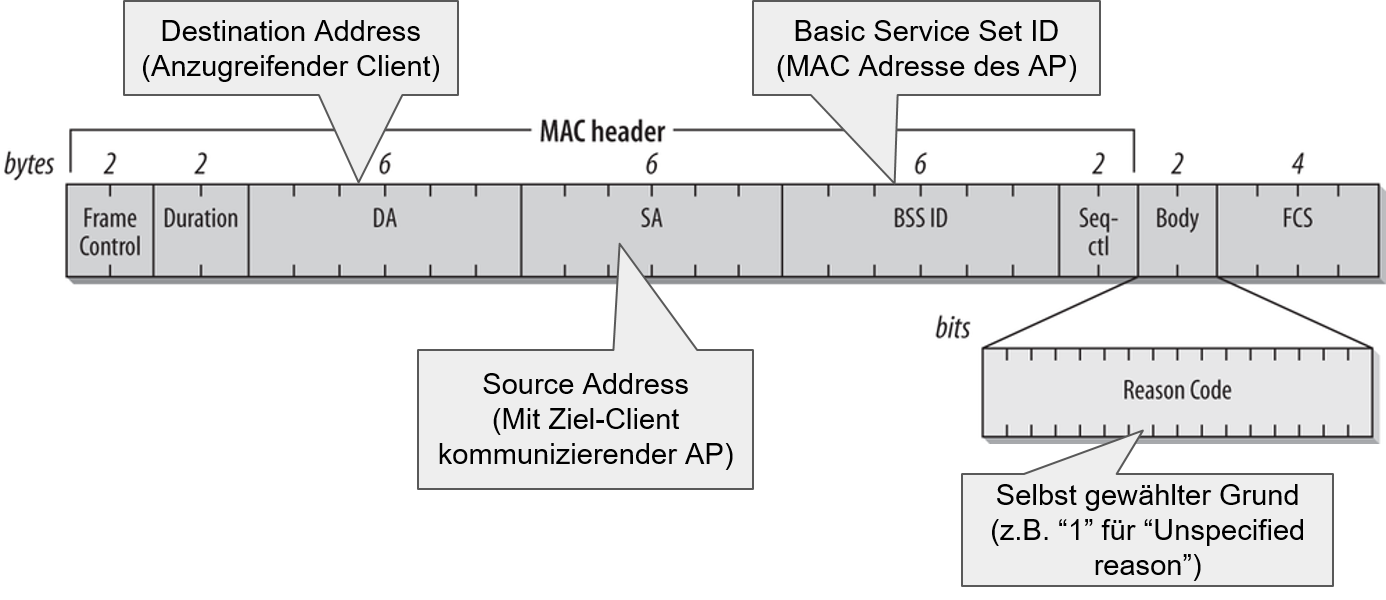
\includegraphics[width=0.7\textwidth]{graphics/deauth-attack}
	\caption[Deauthentication-Frame]{Abbildung eines Deauthentication-Frames~\cite{deauthframe}.}
	\label{fig:deauth-attack}
\end{figure}

Gemäß Spezifikation entspricht in Netzwerken, welche eine Authentifizierung erzwingen, eine Deauthentifizierung einer Disassozierung (durch ein Disassociation-Frame herbeigeführte Verbindungsaufhebung)\footcite[S. 74, S. 442]{ieee802.11}. In einen einem Versuch gegen ein mit \textit{macOS 10.12.4} betriebenes Gerät konnten wir zeigen, dass -- auch wenn der Name es nicht suggeriert -- die Verwendung von Disassociation-Frames für diesen Angriff ebenfalls geeignet ist.

\paragraph{Durchführung}
Zur Durchführung des Deauth-Angriffs müssen zwei Voraussetzungen erfüllt sein: 
\begin{itemize}
	\item der Client ist mit einem AP des Zielnetzwerks verbunden; dieses operiert nach IEEE 802.11
	\item der Angreifer befindet sich in Reichweite zu Client und dessen AP
\end{itemize}

Wie für alle in dieser Arbeit beschriebenen, praktischen Angriffe und Evaluationen wird ein WLAN-Chipset benötigt, dessen Treiber kompatibel mit der \texttt{aircrack-ng}-Suite sind. 
Zunächst versetzt der Angreifer sein Netzwerkinterface (z.B. \texttt{wlan0}) in den \enquote{Monitor-Mode}\footnote{Im Monitor-Modus verarbeitet das Interface alle eingehenden Pakete, nicht nur solche, die an die MAC-Adresse des Empfängers gerichtet sind oder als Broadcast verteilt werden.} und beendet interferierende Hintergrundprozesse:

\begin{Verbatim}
	airmon-ng check kill
	airmon-ng start <Interface im Monitor-Mode>
\end{Verbatim}

Dies ermöglicht das Überwachen des Netzwerkverkehrs und das aussenden eigens erstellter Frames.
Um potentielle Handshakes und andere Pakete aufzuzeichnen verwendet der Angreifer \texttt{airodump-ng}:
\begin{Verbatim}
	airodump-ng -c <Ch> --bssid <AP-MAC> -w <Dateiname> <Interface>
\end{Verbatim}
Ist der Channel nicht bekannt, so kann \texttt{airodump-ng} auch \enquote{Channel-Hopping} betreiben. 
Dies führt in der Praxis jedoch verständlicherweise zu Paketverlusten, weshalb es sich empfiehlt, den Channel vorher in Erfahrung zu bringen. Das Flag \texttt{--bssid} ist optional und dient als Filter. Es verhindert, dass Pakete von anderen APs aufgezeichnet werden und kann somit die nachträgliche Analyse erleichtern und die Datenmenge kleiner halten. Der Einsatz empfiehlt sich womöglich auch aus rechtlicher Perspektive.

Sind die MAC-Adressen des Clients und des AP bekannt startet der Angreifer mit Hilfe von \texttt{aireplay-ng} den Deauth-Angriff: 
\begin{Verbatim}
	aireplay-ng -0 <Anzahl> -a <AP-MAC> -c <Client-MAC> <Interface>
\end{Verbatim}
Das Flag \texttt{-0} kennzeichnet dabei den Deauth-Angriff.
Via \texttt{<Anzahl>} kann spezifiziert werden, wie viele Deauthentication-Frames an das Ziel gesendet werden.
In unseren Versuchen hat sich gezeigt, dass es meistens mehrerer Deauthentication-Pakete bedurfte, um den Client tatsächlich zu einem kurzzeitigen Verlassen des Netzwerkes zu bewegen. Die Wahl der Anzahl hat sich hierbei als Gratwanderung herausgestellt: werden zu wenig Pakete versendet führt der Client keine erneute Authentifizierung durch -- werden jedoch zu viele Pakete versendet, so konnten wir beobachten wie das Endgerät sich mit einem eigentlich niedriger priorisiertem Netzwerk verbunden hat, da ihm einer erneuter Verbindungsaufbau anscheinend nicht möglich erschien. Ein Wert von 20 hat sich in unseren Versuchen als zielführend erwiesen.
Ein Nachteil dieses Ansatzes ist, dass \texttt{aireplay-ng} mit dem Aussenden der Deauthentication-Frames wartet bis es einen Beacon-Frame des Access-Points erhalten hat -- eine technische Notwendigkeit hierfür besteht unserer Ansicht nach nicht.
Alternativ kann die Deauthentifikation mit wenigen Zeilen Python-Code unter Verwendung der Bibliothek \texttt{Scapy} durchgeführt erden.

\begin{minted}[breakbytoken,breaklines]{python}
	import scapy.all as scapy
	# Construct a deauth packet, subtype 12 
	# is the 802.11 code for a deauthentication-frame
	# bssid is equivalent to the MAC of the AP
	p = scapy.RadioTap() / scapy.Dot11(type=0, subtype=12, addr1=clientMac, addr2=bssid, addr3=bssid) / scapy.Dot11Deauth(reason=1)
	scapy.send(p)
\end{minted}

Nach dem Angriff wird die eingangs gestartete Netzwerkaufzeichnung mit \texttt{airodump-ng} gestoppt, um den Dump mithilfe eines geeigneten Tools, zum Beispiel \texttt{Pyrit}, zu analysieren. Dieser Schritt ist optional, die schnelle Verifikation womöglich jedoch hilfreich\footnote{Wurde die MAC-Adresse des Access-Points nicht beim Aufzeichnen des Verkehrs spezifiziert sollte sie nun mit dem Flag \texttt{-b} festgelegt werden.
Andernfalls wird \texttt{Pyrit} für eventuell weitere aufgezeichnete Handshakes von anderen Netzwerken positiv antworten.}: 
\begin{Verbatim}
	pyrit -r <Dump-Name> -b <AP-MAC> analyze
\end{Verbatim}
Ein im Rahmen der Arbeit geschriebenes Python-Skript, welches unter Anderem die oben beschriebenen Schritte automatisiert, findet sich auf \textit{GitHub}\footnote{\href{https://github.com/kastel-wpa2/deauth-tool/blob/master/deauth_jammer.py}{https://github.com/kastel-wpa2/deauth-tool/blob/master/deauth\_jammer.py}}. Ein ebenfalls für diese Arbeit gebautes Tool nutzt unter anderem dieses Skript, um Deauth-Angriffe und das vorangehende Scannen des Netzwerkverkehrs komfortabel über eine Weboberfläche zu ermöglichen\footnote{\href{https://github.com/kastel-wpa2/deauth-tool/blob/master/tool.py}{https://github.com/kastel-wpa2/deauth-tool/blob/master/tool.py}}.
Der Versuch des Brechens des erlangten Handshakes wird in Unterkapitel~\ref{subs:cracking} erläutert.

\subsubsection{\enquote{Evil-Twin}-Angriff}\label{subs:evil-twin-attack}
Ein Nachteil des Deauth-Angriffs ist, dass sowohl Client als auch AP in Reichweite des Angreifers sein müssen (\enquote{on-site}), um den Handshake zwischen beiden abfangen zu können. Der Evil-Twin-Angriff als \enquote{off-site}-Attacke hebt diese Beschränkung auf. Die Idee hierbei ist, einen AP zu imitieren, der einem dem Client bekannten Netzwerk angehört. Auf diese Weise wird der Client zur Durchführung eines Handshakes verleitet, auch wenn das eigentliche Netzwerk nicht in Reichweite ist. 
%Je nach Quelle überlappt der Evil-Twin Angriff mit dem des \textit{Rogue-Access-Points} -- teilweise werden die Begriffe auch synonym verwendet.\\
%TODO: würde ich raus nehmen... klingt blöd und die einzigen die das hier lesen werden wissen was ein evil twin ist
Betrachtet man den Ablauf des Handshakes (siehe Unterkapitel~\ref{subs:handshake}), so stellt man fest, dass die für einen Bruteforce-Angriff wichtigen Elemente keines vollständigen Handshakes bedürfen. Benötigt werden lediglich folgende Informationen:
\begin{itemize}
	\item SSID des Netzwerkes 
	\item MAC-Adressen der beiden Kommunikationspartner
	\item \textit{ANonce} aus Schritt 1
	\item \textit{SNonce} inklusive \textit{MIC} aus Schritt 2
\end{itemize}
Die Parameter, die vom AP übermittelt werden, unterliegen keinerlei Schutz und werden nicht auf Authentizität geprüft.
Der Angreifer kann demnach die ANonce und MAC-Adresse beliebig wählen und den Handshake bis zu Schritt zwei durchführen.
Um die übrigen Parameter zu erhalten (SNonce inklusive MIC) muss der Angreifer dem Client ein authentisches, ihm bekanntes Netzwerk vortäuschen -- den \enquote{Evil-Twin}. In der Praxis ist meist eine bekannte SSID und Sicherheitskonfiguration ausreichend. Letztere entspricht einer der folgenden Möglichkeiten (Unterkonfigurationen nicht betrachtet): Open (kein Schutzverfahren), WEP, WPA-PSK, WPA-Enterprise, WPA2-PSK, WPA2-Enterprise.
Die Anzahl der in der Praxis gängigen Konfigurationen ist sehr begrenzt, der Angreifer kann dementsprechend einfach alle populären Konfigurationen durch einen eigenen, virtuellen AP abdecken. Ist das Zielnetzwerk bekannt (und somit auch die SSID), so ist der Evil-Twin einsatzbereit.

Oft ist jedoch ein konkreter Client Ziel des Angriffs und nicht ein bestimmtes Netzwerk, wenn das Ziel bspw. die Kontrolle von dessen Kommunikation via Man-in-the-Middle-Methoden ist. Prinzipiell sind dem Angreifer die dem Client bekannten Netzwerke verborgen, sofern er nicht gerade aktiv mit diesen kommuniziert.
An dieser Stelle kommen die in Abschnitt~\ref{subs:probes} beschriebenen Probe-Requests in Spiel, die je nach Client kontinuierlich gesendet werden.
Aus diesen kann der Angreifer die SSIDs bekannter Gegenstellen auslesen und gegebenenfalls mehrere APs starten.

Auf diese Art und Weise ist es möglich automatisiert und in kurzer Zeit viele Handshakes für viele verschiedene Netzwerke einzusammeln. Diese dienen dann als Grundlage für einen Angriff in die Breite: Anstelle von komplexen Passwörtern als Kandidaten  für den Bruteforce-Schritt zu wählen, werden nur solche mit einer vergleichsweise hohen Wahrscheinlichkeit verwendet -- jedoch gegen viele Handshakes. Die Annahme dahinter ist, dass wichtige Netzwerke zwar gut gewählte Passwörter verwenden -- die meisten Endgeräte jedoch auch schon mit schlecht geschützten \enquote{Café-WLANs} verbunden waren.

Liegt der Fokus auf der gezielten Kompromittierung eines bestimmten Nutzers, so hängt die Sicherheit der WLAN-Verbindung nun von der Komplexität des schwächsten PSKs ab. Geht es um den Zugriff auf ein bestimmtes Netzwerk, so ist diese Suche nach der \enquote{lowest hanging fruit} nicht zielführend.

\paragraph{Durchführung}
Für den Evil-Twin Angriff bietet die \texttt{aircrack-ng}-Suite zwei mögliche Herangehensweisen, die folgend näher beleuchtet werden sollen.
Zunächst muss, wie beim Deauth-Angriff bereits beschrieben, das Netzwerkinterface in den Monitor-Mode versetzt werden.
Weiß der Angreifer im Vorfeld für welche SSID er den Evil-Twin öffnen möchte, so kann er dafür den folgenden Befehl verwenden:
\begin{Verbatim}
	airbase-ng start --essid <SSID> -Z 4 -F <Dateiname> <Interface>
\end{Verbatim}

Durch das Flag \texttt{-Z 4} wird sich der Evil-Twin als AP eines WPA2-PSK geschützten Netzwerks ausgeben.
Mithilfe von \texttt{-F <Dateiname>} wird der Netzwerkverkehr zwischen dem Evil-Twin und den Clients mitgeschnitten.
Versucht sich ein Client nun mit dem Evil-Twin zu verbinden, so wird der Handshake bis zu Schritt zwei durchgeführt und anschließend abgebrochen.
Dies äußert sich beim Client in Form einer Fehlermeldung wie zum Beispiel: \enquote{Fehler bei der Authentifizierung}. \\

\begin{figure}[ht]
	\centering
	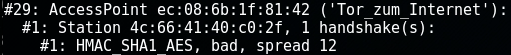
\includegraphics[width=0.7\textwidth]{graphics/pyrit_analyze}
	\caption[Pyrit]{Auch dem mitgeschnittenen Handshake sieht man an, dass es sich nur um einen \enquote{halben Handshake} handelt -- der obenstehende Aufruf von \texttt{pyrit} markiert ihn als \enquote{Bad}, da er nicht erfolgreich durchgeführt wurde. Für einen Angriff eignet er sich dennoch.}
\end{figure}
\FloatBarrier

Kennt der Angreifer keine seinem Ziel bekannten SSIDs, so kann er das \texttt{-P}-Flag verwenden:
\begin{Verbatim}
	airbase-ng start -P -Z 4 <Interface>
\end{Verbatim}

\texttt{Airbase-ng} wird nun auf dem ausgewählten Interface Probe-Requests von Clients auswerten, um automatisch Evil-Twins mit der vom Angreifer spezifizierten (Sicherheits-)Konfiguration zu erzeugen.
Es empfiehlt sich, gleichzeitig einen \texttt{airodump-ng} Prozess zu starten, welcher den Verkehr des Evil-Twins separat aufzeichnet.
Dies hat den Hintergrund, dass die Aufzeichnung von \texttt{airbase-ng} ohne spezifizierte SSID via \texttt{--essid} Flag \texttt{default} als Netzwerknamen verwendet -- anstelle des Wertes aus dem Probe-Request. Dies führt in späteren Schritten zu Problemen, denn ohne gültige SSID werden Handshakes unbrauchbar, da diese in die Berechnung des PMK mit einfließt (und von \texttt{aircrack-ng} automatisch aus dem Dump extrahiert wird).

\subsection{Handshake-Bruteforcing}\label{subs:cracking}
Liegen valide Handshake-Mitschnitte vor, so kann der Angreifer versuchen den PSK offline zu brechen.
Dafür spielt er die Schritte, die Client und AP während des Handshakes durchführen, lokal nach und wählt in jeder Iteration einen neuen Passwortkandidaten.
Die Vorgehensweise entspricht folgendem Algorithmus (siehe auch Abbildung~\ref{fig:wpa2handshake}):
\begin{enumerate}
	\item Berechne $\mathsf{PMK} = \mathsf{PBKDF2}(\mathsf{SSID}, \mathsf{PSK}, 4096, 256)$
	\item Verwende die aufgezeichneten Noncen und berechne damit \\$\mathsf{PTK} = \mathsf{PRF}(\mathsf{Client-MAC},  \mathsf{Access-Point-MAC}, \mathsf{SNonce}, \mathsf{ANonce}, \mathsf{PMK})$
	\item Bilde den $\mathsf{MIC}$ über den $\mathsf{PTK}$-Kandidaten und vergleiche ihn mit dem aufgezeichneten $\mathsf{MIC'}$
	\begin{enumerate}
		\item $\mathsf{MIC} \neq \mathsf{MIC'}$: Neustart von Schritt 1
		\item $\mathsf{MIC} = \mathsf{MIC'}$: Kollision gefunden, Handshake erfolgreich gebrochen
	\end{enumerate}
\end{enumerate}
Der Großteil des Rechenaufwands lässt sich auf das Bilden des PMKs in Schritt 1 durch $4096$ Runden PBKDF2 zurückführen. Ein AP muss diese Rechnung nur einmal durchführen, da sie lediglich von statischen Eingaben abhängt. %Rechenaufwand ist nicht durch die 4096 Runden "immens", sondern durch den großen Passwortraum
Des Weiteren kann nur sehr selten auf vorab generierte PMK-Listen zurückgegriffen werden, da der PMK auch von der SSID des Netzwerkes abhängig ist. Solche Listen existieren, allerdings nur für die häufigsten SSIDs. Als Tool zu ihrer Erzeugung sei hier \texttt{coWPAtty} genannt.

\paragraph{Durchführung}
Es existieren verschiedenste Tools und Online-Services zum Brechen von WPA2-PSK Handshakes, deren Funktionsweise letztlich immer dieselbe ist.

In dieser Arbeit werden die Beispiele mit \texttt{aircrack-ng} (als Teil der gleichnamigen Suite) gezeigt. Erwähnt seien jedoch noch die Programme \texttt{oclhashcat} bzw. \texttt{cudahashcat}, welche durch den Einsatz der massiven Parallelität moderner GPUs eine deutlich höhere Hashes/Sekunde-Rate ermöglichen sowie \texttt{John The Ripper}, welches auch unter Microsoft Windows arbeitet. Im Gegensatz zu \texttt{aircrack-ng} unterstützen diese eine Vielzahl weiterer Algorithmen neben den für WPA2-PSK benötigten.\\

\texttt{Aircrack-ng} benötigt zum Brechen ein Mitschnitt, der die ersten zwei Schritte des WPA2-PSK Handshakes enthält.
Weiterhin ist eine Passwortliste erforderlich die PSK Kandidaten enthält, welche \texttt{aircrack-ng} für den aufgezeichneten Handshake prüfen soll. Alternativ können diese über die Standardeingabe hineingereicht werden.
\begin{Verbatim}
	aircrack-ng -w <Passwortliste> -b <AP-MAC> <Capture> # mit Liste
	crunch ... | aircrack-ng -w - -b <AP-MAC> <Capture> # über stdin
\end{Verbatim}
\texttt{Crunch} ist hierbei ein Tool zur Generierung von Passwortkandidaten auf Basis bestimmter Vorgaben.
Sofern während der Aufzeichnung sichergestellt wurde, dass ausschließlich Verkehr des gewünschten Funkzelle aufgezeichnet wurde, so kann das Flag \texttt{-b} verworfen werden.

\begin{figure}[ht]
	\centering
	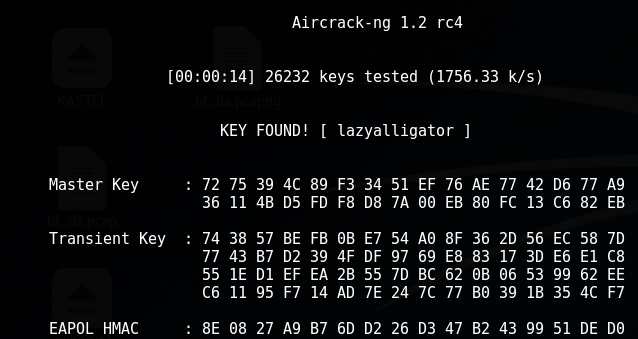
\includegraphics[width=0.7\textwidth]{graphics/aircrack_success}
	\caption[Aircrack-ng]{\texttt{aircrack-ng} hat den gültigen PSK gefunden}
\end{figure}

\FloatBarrier

\newpage

\section{Feldstudie}
Um die Praktikabilität der Angriffe grundlegend zu verifizieren, haben wir bisher gemachte Annahmen hinsichtlich erfüllter Voraussetzungen effizienter Angriffe (z.B. das Aussenden von Probe-Requests durch in Clients) in mehreren Feldstudien überprüft.

Hierfür wurde der Netzwerkverkehr in verschiedenen Umgebungen, sowie das Verhalten von Endgeräten im Falle eines Angriffs, analysiert.
Den folgenden Fragen wurde nachgegangen:
\begin{itemize}
	\item Welche Endgeräte senden in welcher Frequenz Probe-Requests aus?
	\item Wie anfällig sind Endgeräte bezüglich des Evil-Twin Angriffs?
	\item Können Deauth-Angriffe im eigenen Netzwerk erkannt werden bzw. von regulärem Netzwerkverkehr unterschieden werden?
\end{itemize}

Es wurden verschiedene, zur Verfügung stehende Smartphones und Notebooks unterschiedlicher Hersteller auf ihr Verhalten geprüft:
\begin{itemize}
	\item Nokia Lumia 530 (Windows Phone 8.1)
	\item Elephone P9000, Samsung Galaxy S7 Edge, Samsung Galaxy S6 Edge (Android 6)
	\item Lenovo Thinkpad T550 (Windows 10)
	\item Apple MacBook Pro 15 (Mid 2015), Apple MacBook Pro 13 (Mid 2014) (macOS 10.12)
\end{itemize}

\subsection{Detektion von Deauth-Angriffen}
Zwar hängt die Durchführbarkeit eines Deauth-Angriffes nicht von seiner Nachweisbarkeit ab -- der Nutzen womöglich schon. Ist der Angriff offensichtlich und bspw. von einem (besseren) Router sicher detektierbar, so wird ein mitgeschnittenes Passwort u. U. sehr schnell durch ein neues ersetzt. Allerdings dürfte bereits dies schmerzhaft für den Betreiber des Netzes sein.

Da keines der getesteten Endgeräte Schutzmechanismen gegenüber dem Deauth-Angriff aufweist, verzichten wir auf eine ausführliche Beschreibung und fokussieren uns auf dessen Erkennung auf Netzwerkebene. Allerdings wäre die Detektion auf dem attackierten Gerät selbst am sinnvollsten, denn die Vermeidung eines erneuten Handshakes obliegt letztlich diesem. Zudem kann ein Angriff durchaus so ausgeführt werden, dass der AP keine Chance hat, die Deauthentication-Frames überhaupt zu empfangen.
Ein Angreifer könnte in einem aufwendigeren Szenario seine Position zum Senden der Deauthentication-Frames\footnote{Wie in~\ref{subs:deauth-attack} erwähnt eignen sich auch Disassociation-Frames für die Durchführung dieses Angriffs} so wählen, dass die Reichweite den AP nicht mehr umfasst und mit einem zweiten Empfänger, welcher sowohl in Reichweite des Clients als auch des APs ist, den Handshake mitschneiden.
Dies würde auch auf der Erkennung von Anomalien basierende Ansätze wie den in \cite{cheema2011deauth} beschriebenen ins Leere laufen lassen. Wie plausibel eine solche Anomalieerkennung jedoch für das einfache Angriffsmodel erscheint, haben wir mit zwei Messungen in unterschiedlichen Umfeldern in Erfahrung bringen wollen:
\begin{enumerate}
	\item \textbf{WPA2-Personal Heimnetzwerk} mit einem (Endverbraucher-)AP und 8 Teilnehmern, die sich selten aus der Reichweite des Access-Points entfernen
	\item \textbf{WPA2-Enterprise Firmennetzwerk} mit 3 (Enterprise-)APs und ca. 30 Teilnehmern, die sich häufig zwischen den einzelnen Access-Points bewegen
\end{enumerate}
Aus den Merkmalen des Verkehrs, wie beispielsweise Häufigkeit und Reason-Code der Deauthentication-Frames, können wir Eigenschaften ableiten mit denen wir den Deauth-Angriff bezüglich seiner Praxistauglichkeit bewerten können.\\

Im Heimnetzwerk konnte selbst nach 24 Stunden des Aufzeichnens kein Deauthentication-Frame beobachtet werden. Dies ist vermutlich darauf zurückzuführen, dass bei einem AP in einem Heimnetzwerk weder das Verschieben von Clients zwischen APs möglich, noch mit dem Verfall einer Zugangsberechtigung zu rechnen ist.

Im Firmennetzwerk hingegen wurden ca. 2 Deauthentication-Frames pro Minute detektiert.
Hierbei sind ausschließlich die folgenden Reason-Codes aufgetreten (wobei \enquote{STA} als Abkürzung für \enquote{Station} steht und einen Client beschreibt):
\begin{itemize}
	\item 1: \enquote{Unspecified reason}
	\item 2: \enquote{Previous authentication no longer valid}
	\item 6: \enquote{Class 2 frame received from nonauthenticated STA}
	\item 8: \enquote{Disassociated because sending STA is leaving (or has left) BSS}
\end{itemize}
Auffällig war ebenfalls, dass die Access-Points bis zu 5 Deauthentication-Frames in einem Stoß gezielt an einen Client versendet haben.
Dieses Verhalten kann dem Angreifer dabei helfen seinen Angriff zu verschleiern.
So kann er zum Beispiel den Netzwerkverkehr für kurze Zeit analysieren um zu erkennen, mit welcher Frequenz und mit welchen Reason-Codes die Frames von den Access-Points im Zielnetzwerk versendet werden.
In einem Firmennetzwerk ist somit der Deauth-Angriff als praktikabel und auch subtil zu bewerten unter der Annahme, dass der Angreifer die nötige Zeit aufwendet um seinen Angriff entsprechend den Gegebenheiten anzupassen.

Der Deauth-Angriff ist für den Client selbst kaum nachvollziehbar: es kommt lediglich zu einem kurzen Abbruch der Verbindung zum Access-Point ($<< 1$ Sekunde), bevor die erneute Authentifizierung abgeschlossen wurde. Selbst wenn der Nutzer den Angriff bemerkt -- den erneuten Handshake wird er nicht verhindern können.\\

Es lässt sich abschließend sagen, dass eine Anomalieerkennung in einem Heimnetzwerk, zumindest diesem Experiment zu Folge, gut funktionieren würde. Den Aufwand sowie den höheren Kostenfaktor eines entsprechenden Routers dürften die Anwender für ihr Heimnetz allerdings scheuen. In Firmennetzen wäre dies womöglich ein geringeres Problem. Router könnten Alarm schlagen, sobald sie Deauthentication-Frames bemerken, welche sie nicht selbst gesendet haben. Die Variante von zusätzlicher Hardware, welche Anomalien erkennt, dürfte nur sehr unscharfe Ergebnisse liefern.\\

Der Nutzen einer zentralen Detektion ist jedoch weiterhin fraglich, denn letztlich kann nur der Client die erneute Authentifizierung verhindern. Da die Endgeräte solche Mechanismen unseren Versuchen zu Folge jedoch nicht implementieren wird gegen Bruteforce-Angriffe lediglich ein komplexes Passwort helfen. Gegen DoS-Attacken stellt dies allerdings keinen Schutz dar.

\subsection{Probing-Verhalten von Endgeräten}\label{subs:praxisprobes}
Um einen Evil-Twin Angriff (effizient) zu ermöglichen benötigt der Angreifer eine oder mehrere SSIDs von Netzwerken, die dem anzugreifenden Endgerät bekannt sind.
Hierfür werden Probe-Requests zu Hilfe gezogen, die Endgeräte periodisch aussenden um bekannte Netzwerke zu detektieren.
Das Aussenden variiert jedoch hinsichtlich Frequenz und Umfang, ist also abhängig vom Endgerät.
Alle Geräte wurden mit der zum jeweiligen Zeitpunkt aktuellsten verfügbaren Betriebssystemversion getestet. Unsere Versuche sollen nicht als Basis für einen Vergleich der verschiedenen Plattformen gesehen werden -- sie sollen allgemeine Schwachstellen qualitativ überprüfen, sie nicht quantitativ in Relation setzen. Dementsprechend wurden die Listen der, den einzelnen Geräten jeweils bekannten, Netzwerke nicht gezielt angeglichen. Der Netzwerkverkehr wurde mithilfe von \texttt{airodump-ng} aufgezeichnet und nachträglich mit eigens entwickelten Python-Skripten unter Verwendung der \texttt{Pyshark}-Bibliothek analysiert und ausgewertet.\\

Das mit Windows 8.1 betriebene Nokia sowie die getesteten Smartphones unter Android 6 wiesen einen ähnlichen Probing-Verlauf auf; in der Spitze konnten bis zu 40 Anfragen pro Minute beobachtet werden.
Auffällig -- jedoch den Erwartungen entsprechend -- war, dass im Falle der getesteten Android-Geräte mit einer größeren Menge an bekannten Netzwerken auch die Anzahl der Probe-Requests zunahm. Versteckte Netzwerke spielten dabei nur eine untergeordnete Rolle.\\

Um Geräte weiterer Hersteller zu analysieren, wurden Probe-Requests in einer stark frequentierten Bahnhofshalle gemessen. Dabei wurde die Auskunftsfreudigkeit von (Android-)Endgeräten bestätigt. Der Rückschluss auf Android als Betriebssystem ist über die Auflösung der MAC-Adresse auf den jeweiligen Hersteller erfolgt\footnote{Ein Rückschluss auf die jeweils eingesetzte Version ist im Allgemeinen nicht möglich.}.
Das mittlerweile gängige Verfahren der MAC-Randomization~\cite{android6changes, windows10wireless}, bei welchem der vom Hersteller kontrollierte Teil der Adresse randomisiert wird um das Tracking von Endgeräten auf Basis ihrer Probe-Requests zu erschweren, wirkt sich hierbei nicht aus -- konnte bei den von uns kontrollierten Geräten jedoch beobachtet werden.
Weiterhin konnte festgestellt werden, dass Android-Geräte eine Tendenz zum schubartigen Aussenden von Probe-Requests aufweisen.
So wurden binnen weniger 100 Millisekunden alle bekannten SSIDs im Netz veröffentlicht.\\

Das Elephone P9000 sendete sogar weiterhin Probe-Requests, obwohl es mit einem Wireless-Netzwerk verbunden war. Dieses Verhalten konnten wir bei dem genutzten Samsung Galaxy S7 Edge nicht beobachten. Dies lässt vermuten, dass Hersteller entsprechende Teile des Netzwerk-Stacks anpassen und dementsprechend allgemein eine große Abweichung hinsichtlich des Verhaltens im Segment der Android-Smartphones bestehen dürfte.
Potenzielle Erklärungen für das Aussenden von Probe-Request trotz bestehender Verbindung könnten dabei sein, dass das Gerät versucht sich über die umgebenden Netzwerke zu lokalisieren, oder dass es hofft, ein stärkeres, bekanntes Netzwerk in Reichweite zu finden.\\

Die Apple-Geräte sowie der mit Windows 10 betriebene Laptop schienen hingegen sparsamer mit Probe-Requests umzugehen -- auf technisch notwendige Probes (zur Detektion versteckter Netzwerke) haben allerdings auch sie sich nicht beschränkt.\\

Abschließend ist zu sagen, dass keines der getesteten Geräte gänzlich auf Probe-Requests verzichtet hat.
Daher ist die Vorbereitung eines Evil-Twin Angriffs als absolut praktikabel einzustufen.

\subsection{Anfälligkeit der Endgeräte gegenüber einem \enquote{Evil-Twin}}
Nachdem festgestellt worden ist, dass mit wenig Aufwand bekannte SSIDs anhand von Probe-Requests ermittelt werden können, sollte geprüft werden, ob die genannten Geräte eventuelle Schutzmechanismen gegen Evil-Twin Angriffe implementieren.\\

Der Testaufbau bestand darin, auf allen oben genannten Endgeräten das WPA2-PSK geschützte Netzwerk mit der SSID \enquote{Tor\_zum\_Internet} bekannt zu machen, bzw. die Zugangsdaten zu hinterlegen.
Anschließend wurde ein passender Evil-Twin mit dieser SSID via \texttt{airbase-ng} gestartet. Es erfolgte dabei keine Konfiguration, die das Internet tatsächlich über den gefälschten AP erreichbar gemacht hätte. Dieser Schritt wäre erst sinnvoll, wenn der PSK bekannt wäre und ein MITM-Angriff durchgeführt werden sollte. Der eigentliche AP von \enquote{Tor\_zum\_Internet} wurde ausgeschaltet um das Off-Site-Szenario zu erreichen.
Die Endgeräte wurden während der Durchführung des Angriffs nicht bedient und waren nicht in Reichweite anderer bekannter Netzwerke.

An dieser Stelle ist es wichtig wiederholt zu erwähnen, dass der Handshake (siehe~\ref{subs:handshake}) im Schritt 3 durch den Evil-Twin abgebrochen wird -- es also nicht zu einer funktionsfähigen Verbindung kommt.
So zeichnete sich das Samsung Galaxy S6 Edge durch ein aggressives Assoziierungsverhalten aus: Mit einer Rate von ca. zwei Authentifizierungen pro Sekunde stach dieses Endgerät besonders heraus.
Wurde ein weiteres Netzwerk bekannt gemacht, dessen AP räumlich jedoch deutlich aufgestellt war, so konnte sogar beobachtet werden, wie das Endgerät von verbundenen AP zum stärker sendendem AP ohne Internetzugang zu wechseln versuchte. 
In diesem Fall konnte der Evil-Twin für einen Denial-of-Service Angriff missbraucht werden -- der Anwender wäre ohne es zu merken nicht mehr online, auch da das Gerät eine mögliche und prinzipiell aktivierte LTE-Verbindung als Rückgriff nicht nutze.

Die übrigen Smartphones haben nach zwei bis vier gescheiterten automatischen Authentifizierungen aufgegeben und sind auf die Nutzung von mobilem Internet zurückgefallen.
Dieses Verhalten wiederholte sich jedoch periodisch in Zeitabständen von 30 bis 60 Sekunden.\\

Es hat sich der Eindruck manifestiert, dass wenn mehrere bekannte Netzwerke in Reichweite sind, die meisten Endgeräte das stärkste Netzwerk auswählen -- nicht nur bei einem initialen Verbindungsaufbau sondern auch bei bereits bestehender Verbindung. Dies erleichtert einen Evil-Twin Angriff, da sich keine zusätzliche Bedingung aus dem aktuellen Status des Opfers ergibt.
Wir konnten dieses Verhalten bei allen Endgeräten Ausnutzen, um sie zur Authentifikation mit dem Evil-Twin zu verleiten.\\

Ist der Typ des Netzwerks vorher nicht bekannt kann der Angreifer, wie bereits erwähnt, mehrere Evil-Twins auf dem Netzwerkinterface öffnen.
Alle getesteten Endgeräte haben sich in diesem Fall mit dem Access-Point mit der passenden Sicherheitskonfiguration verbunden.
Wurde absichtlich eine falsche Konfiguration angeboten, so haben dies lediglich das Windows Phone sowie der Windows 10 betriebene Laptop erkannt und den Nutzer entsprechend gewarnt. %TODO Bild hier
Erstaunlicherweise haben die übrigen Endgeräte sich in einen offenen Evil-Twin ohne jegliche Verschlüsselung locken lassen, womit einem Man-in-the-Middle Angriff Tür und Tor geöffnet wird. Hierdurch entfällt jedwede, eigentlich geforderte implizite Authentifizierung des AP durch Kenntnis des PSK zur Durchführung der Kommunikation.\\

Zusammenfassend ist der Evil-Twin als ein -- wenn auch wenig subtiler -- hochflexibler Angriff zu bewerten. Er kann Off-Site eingesetzt werden, weswegen der reale AP für den Angriff nicht von Nöten ist.
Eigenen Tests nach harmoniert der Evil-Twin Angriff sehr gut mit dem Deauth-Angriff.
So kann ein bereits mit einem anderen Netzwerk verbundener Client so lange deauthentifiziert werden, bis er sich mit dem Evil-Twin verbindet.
Einziger Nachteil bleibt, dass der Evil-Twin in der Umgebung für alle sichtbar ist und somit leicht erkannt werden kann -- dies lässt sich jedoch durch ein \enquote{gezieltes Broadcasting} von Beacon-Frames oder dem Einsatz des Probe-Request-Response Schema von versteckten Netzwerken abschwächen.


\newpage

\section{Ausblick}
In dieser Ausarbeitung wurde gezeigt, wie ein Angreifer mit geringem Hardwareaufwand effizient WPA2-PSK Handshakes zwischen Client und Access-Point erhalten kann, um diese nachträglich mit geeigneten Tools zu brechen.
Befindet sich der Angreifer vor Ort, so kann der Deauthentication-Angriff genutzt werden um einen erneuten Handshake zwischen den beiden Teilnehmern zu forcieren.
In verwalteten Netzwerken, in denen Deauthentication-Frames zum Einsatz kommen, kann dieser Angriff durchgeführt werden, ohne dass der Client die Möglichkeit besitzt eine valide Deauthentifizierung von einer gefälschten zu unterscheiden.
Ist der Handshake gebrochen, so hat der Angreifer mit dem erratenen PSK Zugriff auf das interne Netzwerk. 
Des weiteren lässt sich der komplette Nachrichtenverlauf, der seit dem Handshake aufgezeichnet wurde, nachträglich entschlüsseln.
Dies gilt auch für zukünftigen Netzwerkverkehr anderer Clients unter der Voraussetzung, dass auch hier der Handshake mitgeschnitten wurde.
Da der PSK bekannt und die übrigen Parameter öffentlich sind kann der PTK direkt berechnet werden.
Da keine Schutzmechanismen gegen den Deauthentication-Angriff existieren bedarf es der Erweiterung des Standards um den Deauthentication-Frame zu authentifizieren. %TODO Welcher für WPA2?

Alternativ kann der Angreifer mithilfe des Evil-Twin Angriffs ohne einen echten Access-Point in Reichweite den Client zum Handshake verleiten.
Ein weiterer Vorteil dieses Verfahrens ist, dass gezielt für einen Client mehrere Handshakes für alle bekannten Netzwerke gesammelten werden können, solange er diese via Probe-Requests bekannt gibt.
Um nun beispielsweise einen Man-in-the-Middle Angriff durchzuführen muss der Angreifer nicht etwa einen großen, komplexen Passwortraum explorieren, sondern lediglich das am schwächsten geschützte, dem Client bekannte Netzwerk finden.
Ein Client kann sich schützen, indem er auf dem Endgerät die MAC-Adressen bekannter Access-Points speichert denen er vertraut. 
Damit kann zumindest einem breitflächigen Off-Site Angriff entgegengewirkt werden, denn ist der Angreifer in Reichweite der vertrauten Access-Points kann er deren MAC-Adressen aus verschiedensten Frames extrahieren.
In einem Netzwerk mit vielen Access-Points ist die Pflege dieser Einträge jedoch mühselig und zu aufwändig.
%TODO:Noch irgendwas von wegen Probe Requests sind unnötig

Abschließend ist zu erkennen, dass beide vorgestellten Angriffe auf der Annahme aufbauen, dass Clients mit schwach geschützten Netzwerken verbunden sind und ein mitgeschnittener WPA2-PSK Handshake daher leicht zu brechen ist.
Im Umkehrschluss ist der einzig wirksame Schutz die Verwendung eines starken Passworts oder eines sichereren Handshakes, der sowohl den Client als auch den Access-Point authentifiziert.


%Hinweis, dass über Replay-Attacken mit getrennten Funkstrecken auch ohne Brechen des eigentlichen Handshakes eine Authentifizierung erfolgen kann, diese jedoch nichts nutzt, da die weitere Kommunikation mit PSK erfolgt (Ist das so? Wird kein neuer Schlüssel ausgehandelt?).
%Was kann mit Schlüssel angestellt werden? Wieso sollte man ihn haben wollen? 
%Wie kann ich den Payload einer Nachricht als Evil Twin mitlesen? 

\newpage

\appendix	

\listof{figure}{Abbildungen}

\listof{listing}{Listings}

\section{Literaturverzeichnis}
	\begingroup
	\sloppy
	\printbibliography[heading=none]
	\endgroup

\end{document}